\documentclass[journal,12pt,onecolumn]{IEEEtran}
\usepackage{cite}
\usepackage{caption}
\usepackage{graphicx}
\usepackage{amsmath,amssymb,amsfonts,amsthm}
\usepackage{algorithmic}
\usepackage{graphicx}
\usepackage{textcomp}
\usepackage{xcolor}
\usepackage{txfonts}
\usepackage{listings}
\usepackage{enumitem}
\usepackage{mathtools}
\usepackage{gensymb}
\usepackage{comment}
\usepackage[breaklinks=true]{hyperref}
\usepackage{tkz-euclide} 
\usepackage{listings}
\usepackage{gvv}
%\def\inputGnumericTable{}
\usepackage[latin1]{inputenc} 
\usetikzlibrary{arrows.meta, positioning}
\usepackage{xparse}
\usepackage{color}                                            
\usepackage{array}                                            
\usepackage{longtable}                                       
\usepackage{calc}                                             
\usepackage{multirow}
\usepackage{multicol}
\usepackage{hhline}                                           
\usepackage{ifthen}                                           
\usepackage{lscape}
\usepackage{tabularx}
\usepackage{array}
\usepackage{float}

\usepackage{float}
%\newcommand{\define}{\stackrel{\triangle}{=}}
\theoremstyle{remark}
\usepackage{circuitikz}
\captionsetup{justification=centering}
\usepackage{tikz}

\title{Matrices in Geometry 4.13.42}
\author{EE25BTECH11037 - Divyansh}
\begin{document}
\vspace{3cm}
\maketitle
{\let\newpage\relax\maketitle}
\textbf{Question: }
Let $0<\alpha<\frac{\pi}{2}$ be a fixed angle. If $\vec{P}=\brak{\cos{\theta},\  \sin{\theta}}$ and $\vec{Q} = \brak{\cos{\brak{\alpha - \theta}}, \ \sin{\brak{\alpha - \theta}}}$, then $\vec{Q}$ can be obtained from $\vec{P}$ by
\begin{enumerate}[label=(\alph*)]
    \item clockwise rotation around the origin through an angle $\alpha$
    \item anticlockwise rotation around the origin through an angle $\alpha$
    \item reflection in the line through origin with slope $\tan\alpha$
    \item reflection in the line through origin with slope $\tan\brak{\frac{\alpha}{2}}$
\end{enumerate}

\vspace{2mm}

\textbf{Solution:}
\vspace{1mm}
\\
We know that $\vec{Q}=\myvec{\cos{\brak{\alpha - \theta}} \\ \sin{\brak{\alpha - \theta}}}$ and $\vec{P}=\myvec{\cos{\theta}\\ \sin{\theta}}$\\
We also know that the rotation matrix $\vec{R}=\myvec{\cos\alpha & -\sin\alpha \\ \sin{\alpha} & \cos\alpha}$, where $\alpha$ is anticlockwise.
\\ We can obtain $\vec{Q}$ by
\begin{align}
    \vec{Q}=\vec{R}\vec{P} \implies \vec{Q}=\myvec{\cos\theta\cos\alpha - \sin\theta\sin\alpha \\ \sin\theta\cos\alpha +\cos\theta\sin\alpha   } 
\end{align}
We know from trigonometric identities that
\begin{align}
    \cos{\brak{\alpha-\theta}}=\cos\theta\cos\alpha + \sin\theta\sin\alpha \\\sin{\brak{\alpha-\theta}}=\cos\theta\sin\alpha - \sin\theta\cos\alpha
\end{align}
If we take $\alpha$ clockwise, that is, exchange it with $-\alpha$, we will get the rotation matrix as 
\begin{align}
    \vec{R}=\myvec{\cos\alpha & \sin\alpha \\ -\sin{\alpha} & \cos\alpha}
\end{align}
Thus, the required rotation matrix is $\vec{R}$ using which $\vec{Q}$ can be obtained from $\vec{P}$ by clockwise rotation around the origin through an angle $\alpha $, therefore the correct option is $\brak{a}$\\ 
\vspace{1mm}
Let us plot a graph for $\theta=45^{\degree}$ and $\alpha=30^{\degree}$
\begin{figure}[H]
    \centering
    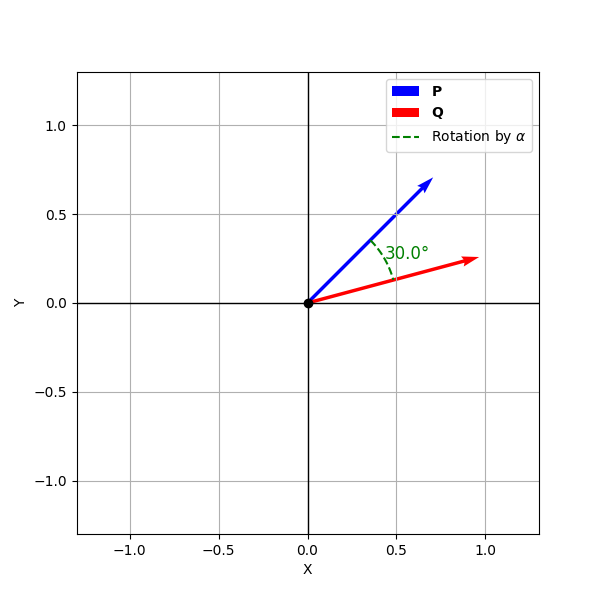
\includegraphics[width=1\columnwidth]{figs/1.png}
    \caption{Graph for 4.13.42, where $\theta=45^{\degree}$ and $\alpha=30^{\degree}$}
    \label{fig:placeholder}
\end{figure}
\end{document}